% This is the aspauthor.tex LaTeX file
% Copyright 2010, Astronomical Society of the Pacific Conference Series

\documentclass[11pt,twoside]{article}
\usepackage{asp2010}
\usepackage{listings}
\usepackage{color}
\definecolor{Red}{rgb}{0.9,0.0,0.1}

\resetcounters

%\bibliographystyle{asp2010}

\markboth{Petr \v{S}koda, Jaroslav V\'{a}\v{z}n\'{y}}{Author's Final Checklist}

\begin{document}
% vylepseny listing z http://texnik.de/TeXnik/listings/listing0.pdf
 \definecolor{hellgelb}{rgb}{1,1,0.8}
 \definecolor{colKeys}{rgb}{0,0,1}
 \definecolor{colIdentifier}{rgb}{0,0,0}
 \definecolor{colComments}{rgb}{1,0,0}
 \definecolor{colString}{rgb}{0,0.5,0}
 \lstset{%
   language={SQL},%
    morekeywords={AND,ASC,avg,CHECK,COMMIT,count,DECODE,DESC,DISTINCT,%
                 GROUP,IN,LIKE,NUMBER,ROLLBACK,SUBSTR,sum,VARCHAR2}%
 }

 \lstset{%
     float=hbp,%
     basicstyle=\ttfamily\small, %
%     identifierstyle=\color{colIdentifier}, %
%     keywordstyle=\color{colKeys}, %
     stringstyle=\color{colString}, %
     commentstyle=\color{colComments}, %
     columns=flexible, %
     tabsize=4, %
     frame=single, %
     extendedchars=true, %
     showspaces=false, %
     showstringspaces=false, %
   numbers=left, %
   numberstyle=\tiny, %
   breaklines=true, %
   backgroundcolor=\color{hellgelb}, %
   breakautoindent=true, %
   captionpos=b%
 }



\title{ASP Author Template}
\author{Petr \v{S}koda$^1$, Jaroslav V\'{a}\v{z}n\'{y}$^2$
\affil{$^1$Astronomical Institute, Academy of Sciences, Ond\v{r}ejov, Czech
Republic}
\affil{$^2$Masaryk University, Faculty of Science, Brno, Czech Republic}}

\begin{abstract}Current data deluge in
astronomy requires applying data mining techniques to extract new
information about the physical nature of celestial objects. The
possibility of cross-matching several surveys via Virtual Observatory
protocols may play a key role in future discoveries. Data mining of
large collections of spectra seems to be one of promising as well as
challenging topics.  We have focused on obtaining new candidates of
H$\alpha$ emission stars using supervised data mining method of
Decision Trees on almost 200,000 spectra in SDSS SEGUE spectral
survey.
\end{abstract}

\section{Process Overview}
Schema of the process is on the Fig.~1. Using SSA protocol the spectra
from Ond\v{r}ejov 2m telescope archive server were acquired based on the list of justified Be stars
obtained from other studies.  Convolution of Ond\v{r}ejov spectra with SDSS
instrumental profile had to be performed to
ensure the compatibility with the lower spectral resolution of SDSS. 
Then the desired features were extracted automatically
from the spectra after the continuum normalisation and H$\alpha$ line
was fitted by appropriate function. The same was done for spectra from
SDSS except the convolution process. Thus the vectors of parameters
characterising the typical Be star H$_\alpha$ emission line were obtained and
subjected to data mining process.
%
%
\begin{figure}[!htbp]
  \begin{center}
    \leavevmode
    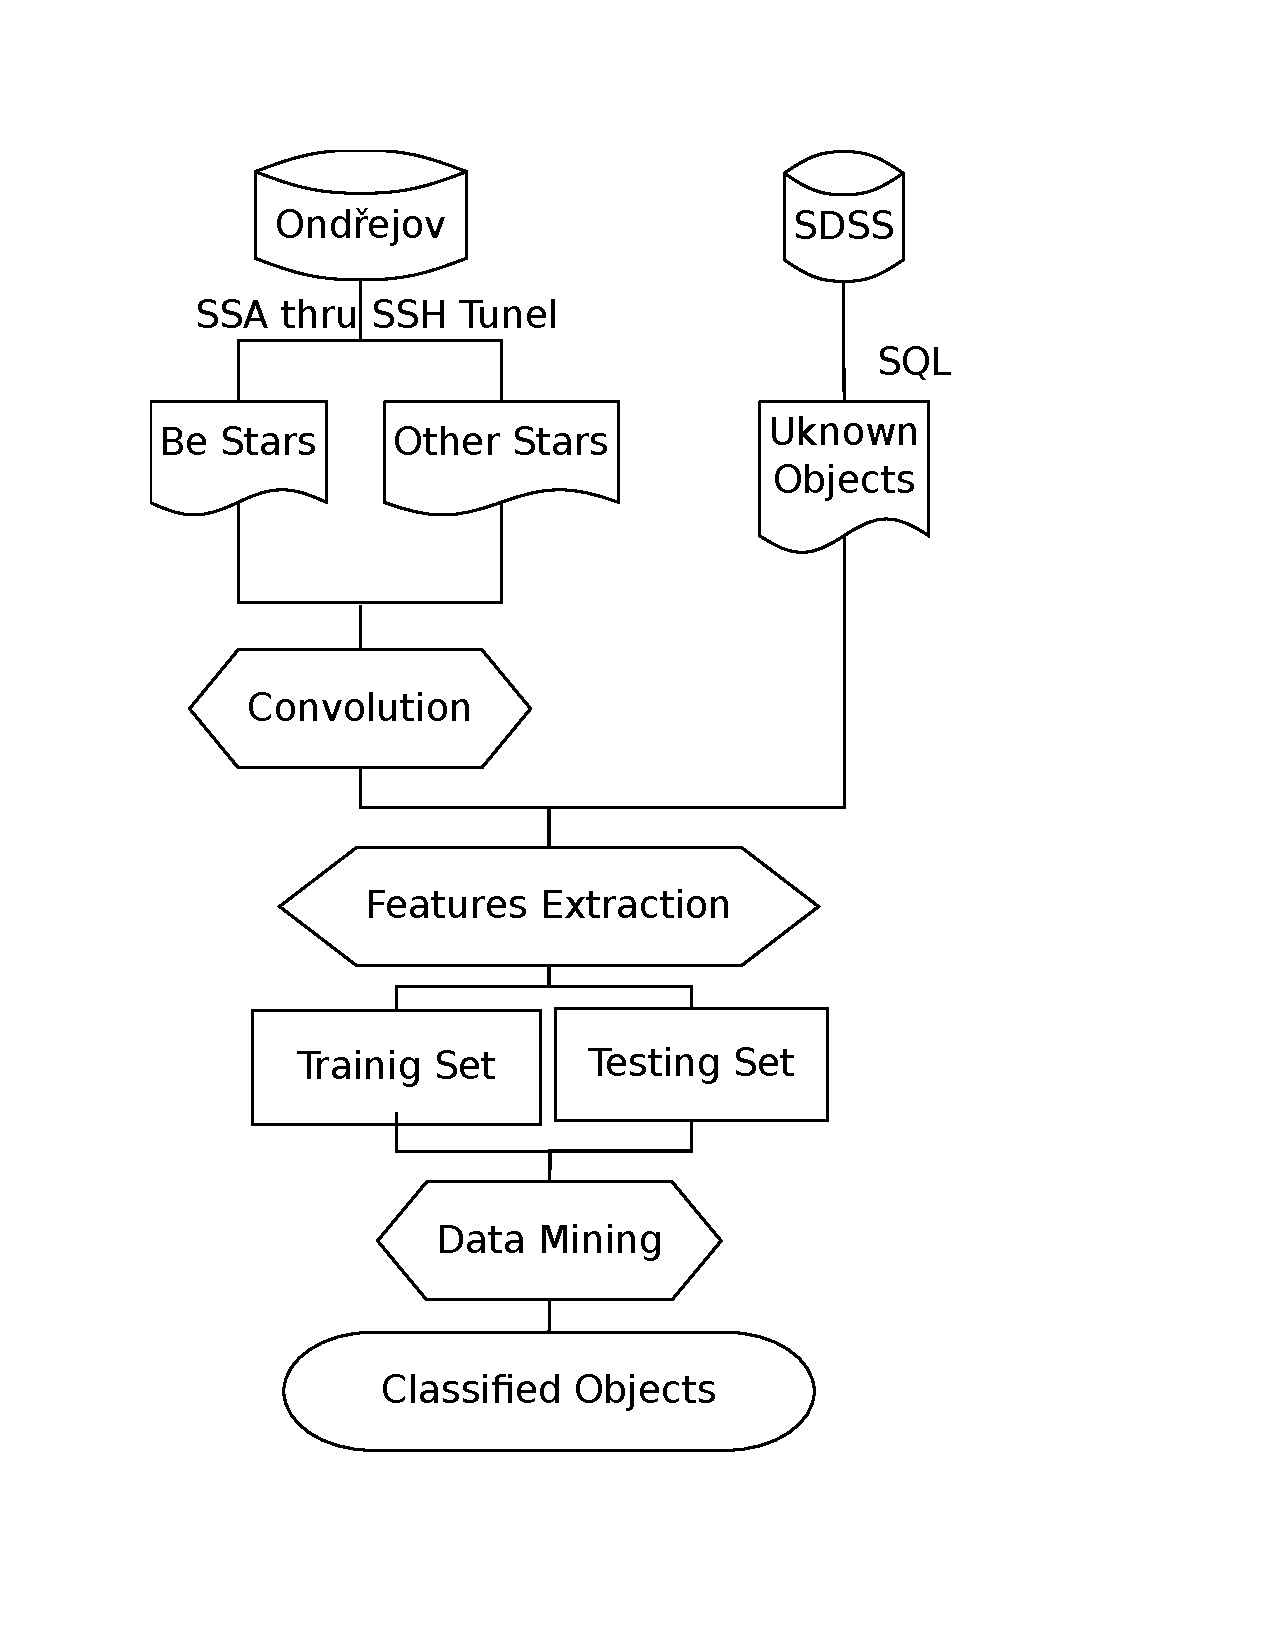
\includegraphics[scale = .4]{flowSpectra}
    \caption{The data mining process overview}
    \label{FigStructure}
  \end{center}
\end{figure}


\section{Degradation of Spectral Resolution}

Spectra from Ond\v{r}ejov Observatory have higher spectral resolution
than SDSS, therefore the degradation of spectral resolution was
applied on them followed by re-binning to the same number of pixels as the
SDSS. So we obtained the training set of Ond\v{r}ejov Be stars spectra looking
similar to  SDSS spectra.

For that purpose convolution in discrete form was used
%
\begin{equation}
  \label{eq:discreteConvolution}
  (f * g)[n]\ \stackrel{\mathrm{def}}{=}\ \sum_{m=-\infty}^{\infty} f[m]\, g[n - m]
\end{equation}
%
An example of this process applied on spectra of Be star 4 Her is on the
Fig.~2. The top figure shows Gaussian function used for convolution
with the spectrum, followed by the original spectrum, then there is a
spectrum after convolution with the Gaussian profile. The last is the
final spectrum after re-binning


\begin{center}
\begin{figure}[!htbp]
  \begin{center}
    \leavevmode
    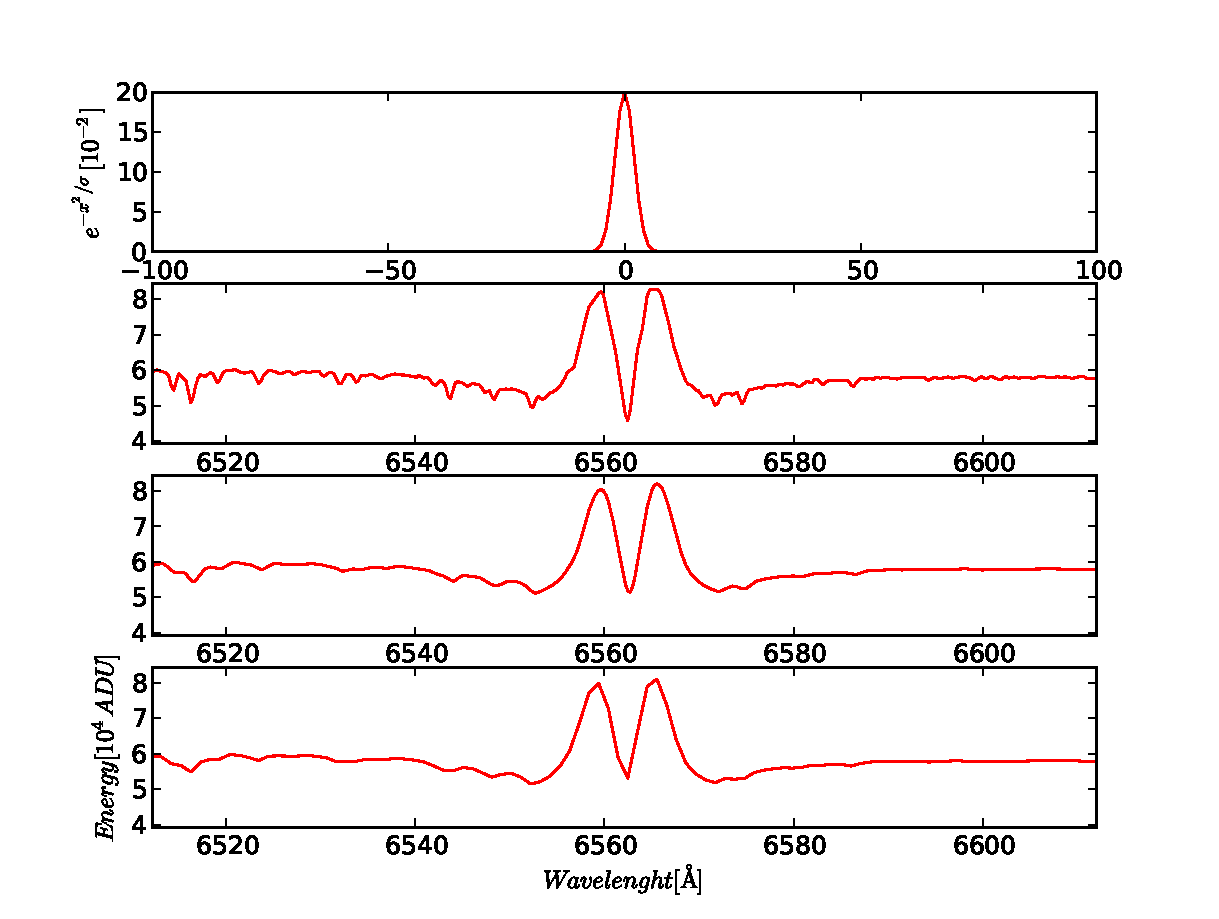
\includegraphics[scale = .6]{convolution}
    \caption{The convolution with SDSS instrumental profile and re-binning applied on Ond\v{r}ejov spectra}
    \label{FigConvolution}
  \end{center}
\end{figure}

\end{center}
%


%
\section{Data Sources}
The spectra obtained with coud\`e spectrograph of Ond\v{r}ejov
Observatory 2m telescope were used as a training sample. Files were
downloaded using SSA protocol. The SSA server is not publicly
accessible outside of the local network of Ond\v{r}ejov observatory.
That is why the SSH tunneling of HTTP protocol was used. Two scripts
for this process were created. First to construct the list of SSA
compliant addresses, the second to analyse acquired response in
VOTable format.

As testing sample the spectra from project SEGUE of SDSS were
selected. This contains 178314 spectra in DR7. A simple SQL query was
used to generate the list of URL links for individual FITS
files. 


\section{Spectral Lines Characteristics}
As parameters for data mining process characteristic values of
H$\alpha$ line were extracted from the spectra. Three parameters were
finally selected. The height and the width of the H$\alpha$ emission
line and median absolute deviation as a characterisation of the noise
level in the spectrum.


\begin{center}
\begin{figure}[!htbp]
  \begin{center}
    \leavevmode
    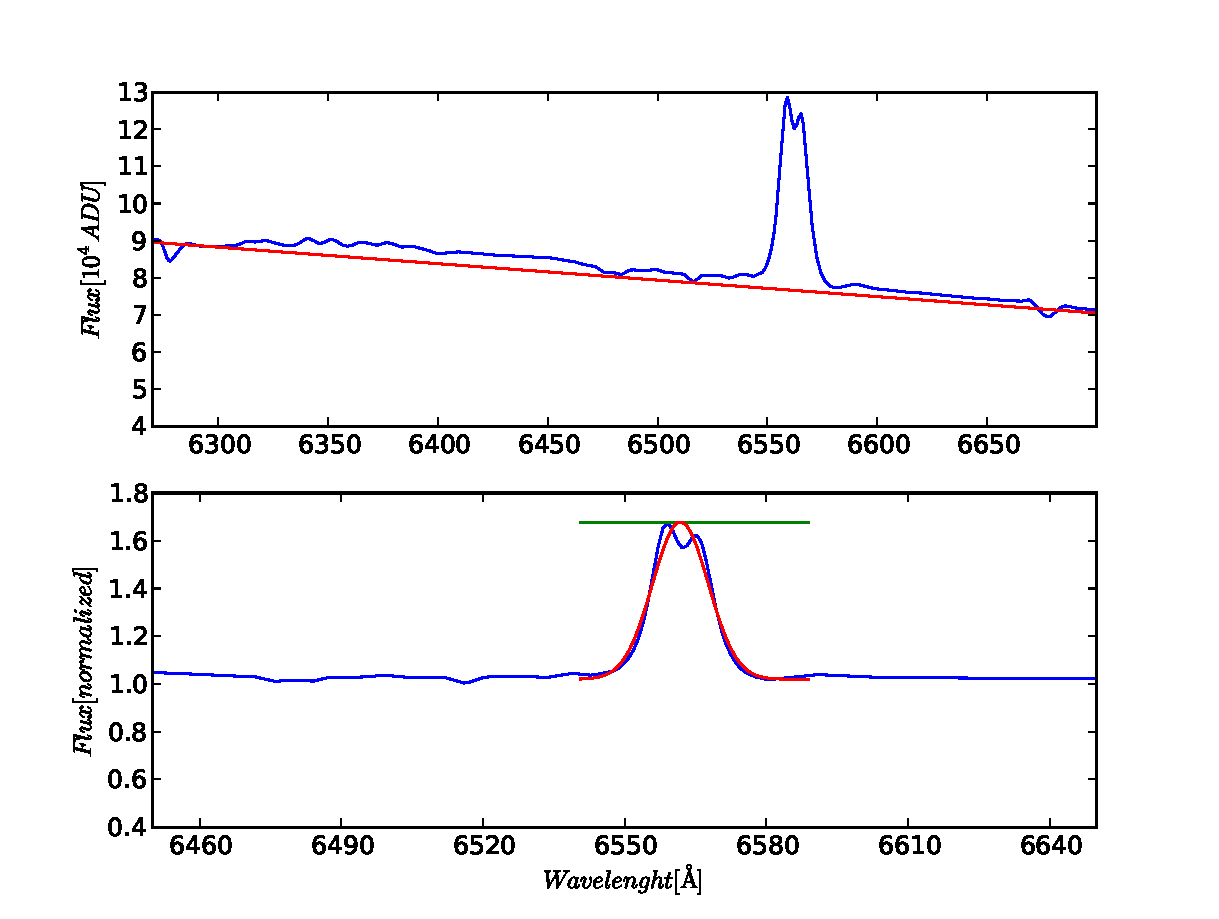
\includegraphics[scale = .6]{figSpecCharCyg60}
    \caption{The normalised spectrum of Be star 60 Cyg. The top figure
      depicts the continuum fit. The bottom figure shows the region
      (width of the green line) used for extraction. The position of
      the line corresponds to the maximum value in the region of
      $50\,\textrm{\AA}$. The Gaussian fit is in red. Although the fit
      is almost perfect, this approach fails to get characteristic
      double peak of the emission line}
    \label{FigConvolution}
  \end{center}
\end{figure}

\end{center}



\section{Data Mining}
The decision tree based classification was performed using Weka software with algorithm
J48, which is the free implementation of algorithm C4.5. The training set had
173 and testing set 178314 items.



\begin{lstlisting}
  === Summary ===
Correctly Classified Instances         145               83.815  %
Incorrectly Classified Instances        28               16.185  %
Kappa statistic                          0.6529
Mean absolute error                      0.1849
Root mean squared error                  0.3652
Relative absolute error                 39.8819 %
Root relative squared error             75.8919 %
Total Number of Instances              173     
\end{lstlisting}

\begin{lstlisting}
  J48 pruned tree
------------------
max <= -0.18843
|   max <= -0.324763: o (46.0/5.0)
|   max > -0.324763
|   |   max <= -0.255475
|   |   |   mad <= 0.004133: o (2.0)
|   |   |   mad > 0.004133: be (13.0/1.0)
|   |   max > -0.255475
|   |   |   mad <= 0.009862: o (10.0)
|   |   |   mad > 0.009862
|   |   |   |   width <= 7.621593: o (3.0/1.0)
|   |   |   |   width > 7.621593: be (2.0)
max > -0.18843
|   mad <= 0.030316
|   |   max <= -0.091726
|   |   |   width <= 5.286489
|   |   |   |   max <= -0.170022: be (2.0)
|   |   |   |   max > -0.170022: o (3.0)
|   |   |   width > 5.286489: be (9.0)
|   |   max > -0.091726: be (76.0)
|   mad > 0.030316
|   |   max <= 6.917615: o (4.0)
|   |   max > 6.917615: be (3.0)
\end{lstlisting}


\parbox{0.999\textwidth}{Fig.~4. The classifier decision tree obtained from data mining process} 
%

%-----------------------------------------------------------------------


\section{Results}

From the 10-fold cross-validation of training-set we estimate the overall
fruitfulness of classification to about 84\%, which is quite good taking into
account specific  double-peak profile  of Be stars and the temporal nature of
their emission episodes. The classifier has identified 1110 Be stars
candidates in SEGUE, however most of them are probably of different nature
(e.g. AGNs, young stellar objects or reduction artifacts). Nevertheless, there
are as well several highly probable  Be stars like the one on Fig.~5.


\begin{center}
\begin{figure}[!htbp]
  \begin{center}
    \leavevmode
    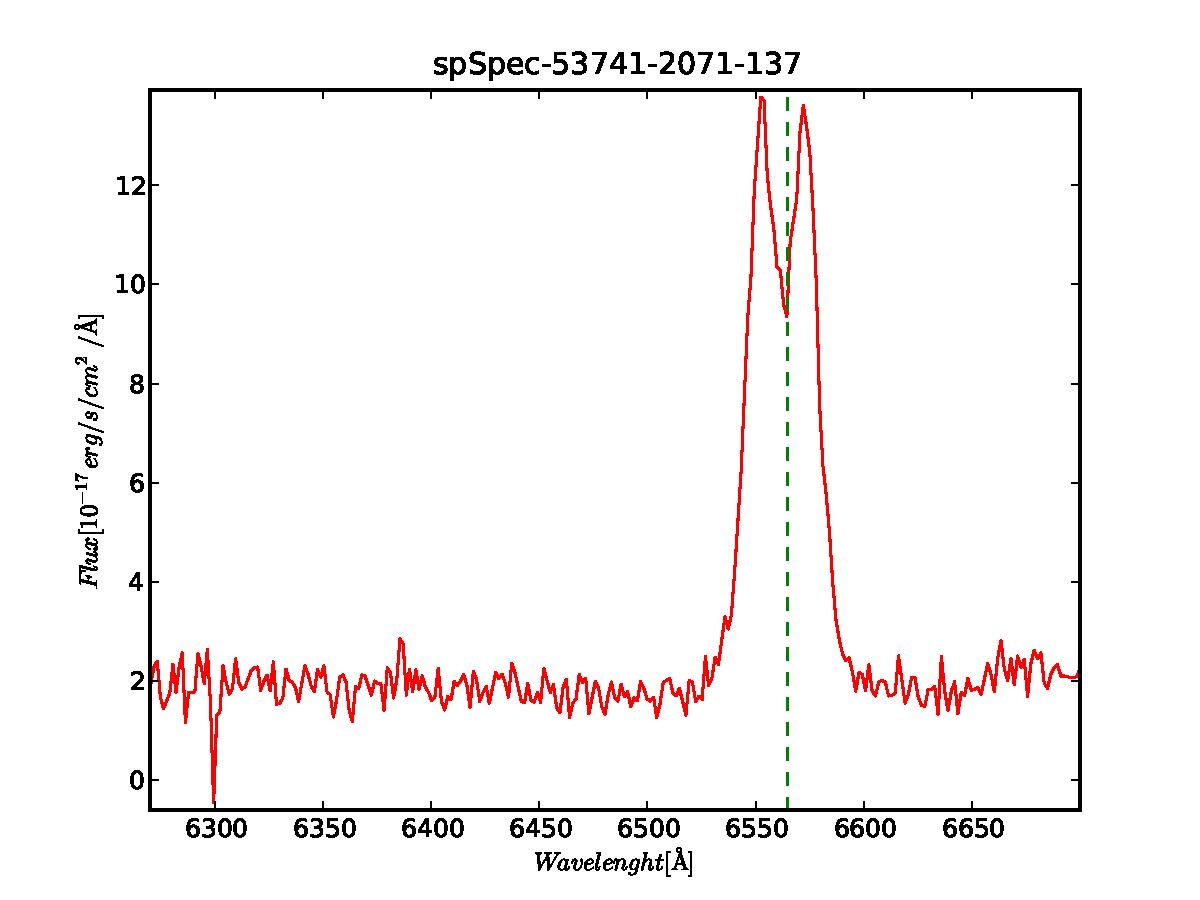
\includegraphics[scale = .6]{result1}
    \caption{The example of candidate Be star found in SDSS
      SEGUE survey using the decision tree shown above.}
    \label{FigConvolution}
  \end{center}
\end{figure}

\end{center}


%
%\vspace{-10mm}
%\begin{center}
%  \resizebox{1.0\hsize}{!}{\includegraphics{result2}}
%\end{center}
%

\section{Spectral Line Parameters}

\textbf{The height of the H$\alpha$ line}

The maximum value in the region of $50\,\textrm{\AA}$ around H$\alpha$
above the linear fit was extracted from the spectrum.

\textbf{The noise level of the spectrum}

The noise in the spectrum contributes to the characteristics of the
spectral lines. As an estimator of the noise level the median
absolute deviation was used. It is defined as:
%
\begin{equation}
  \textrm{mad} = \textrm{median}_{i}\left(\ \left| X_{i} -
      \textrm{median}_{j} (X_{j}) \right|\ \right)
\end{equation}
%
\textbf{The width of the H$\alpha$ line}

The Gaussian function:
%
\begin{equation}
  \label{eq:gauss2}
  f(x) =  1 + e^{- { \frac{(x-x_0)^2 }{ S^2} } }
\end{equation}
%
was fitted to the profile of H$\alpha$ spectral line. 
%
%% First the robust estimators \citep{launer1979robustness} were computed
%% and used as input parameters for leastsq\footnote{"leastsqi"s a
%%   wrapper around MINPACK’s lmdif and lmder algorithms.} method from
%% scipy.opt module, which minimize the sum of squares.
%



\acknowledgements The ASP would like to the thank the dedicated researchers that are publishing with the ASP.

%\bibliography{aspauthor}

\end{document}
